\section{Design and Implementation}
\subsection{User Requirements} 
The requirements for the plug-in were derived from a synthesis of Cognitive Load Theory and specific \gls{neurodivergent} accessibility guidelines, notably the direct 
instructions and visual comfort frameworks identified by \textcite{rocha2025conceptual}.

\begin{table}[H]
    \centering
    \caption{Functional and Non-Functional Requirements for the Accessible \gls{IDE} Plugin}\label{tab:requirements}
    \small
    \begin{tabularx}{\textwidth}{@{} l l X X @{}}
        \toprule
        \textbf{ID} & \textbf{Category} & \textbf{Requirement Description} & \textbf{Theoretical Justification} \\ 
        \midrule
        
        \textbf{FR1} & Interface &
        The system shall provide a single-click \textit{Minimalist Toggle} to simultaneously hide the Activity Bar, Side Bar, Status Bar, and Breadcrumbs. &
        Direct suppression of \gls{EL} through reduction of visual stimuli, supporting inhibitory control and minimising sensory overload in line with Cognitive Load Theory. \\ 
        \addlinespace
        
        \textbf{FR2} & \gls{AI} Support &
        The \textit{Task Architect} shall decompose high-level prompts into a structured checklist of 10 manageable sub-tasks, each containing micro-steps. &
        \Gls{scaffolding} of \gls{IL} to reduce \gls{executive_dysfunction} and \gls{task_initiation} barriers through stepwise decomposition and cognitive \gls{scaffolding} principles. \\ 
        \addlinespace
        
        \textbf{FR3} & Feedback &
        The \textit{Code Explainer} shall intercept compiler errors and provide non-technical bulleted summaries (maximum three points). &
        Reduction of \gls{EL} by converting jargon-heavy diagnostic messages into direct instruction, aligned with split-attention reduction and plain-language accessibility principles. \\ 
        \addlinespace
        
        \textbf{FR4} & Time Management &
        The system shall provide a customisable Pomodoro timer integrated into the dashboard, allowing user-defined focus and break durations. &
        Supports \gls{EF} through temporal externalisation, mitigating \gls{time-blindness} and \gls{hyperfocus} burnout commonly reported in \gls{ADHD} and \gls{ASD} literature. \\ 
        \addlinespace
        
        \textbf{FR5} & Visual Presets &
        The system shall provide at least three predefined typography presets (Standard, Relaxed, Spacious) that simultaneously adjust line height, letter spacing, and font family. &
        Reduces visual stress and improves readability for dyslexic users through evidence-based typography adaptation and visual comfort frameworks. \\ 
        
        \midrule
        
        \textbf{NFR1} & Accessibility &
        The UI must conform to \gls{WCAG} 2.1 Level AA contrast ratios (minimum 4.5:1 for standard text). &
        Ensures inclusive visual accessibility and compliance with recognised accessibility standards. \\ 
        \addlinespace
        
        \textbf{NFR2} & Cognitive &
        The system must provide non-destructive restoration, allowing users to instantly revert all interface changes. &
        Reduces verification anxiety and supports psychological safety by preserving user agency over the environment. \\ 
        \addlinespace
        
        \textbf{NFR3} & Latency &
        \gls{AI}-generated task steps must begin streaming within 2 seconds of request initiation. &
        Minimises interruption-related attentional drift and prevents task-switching overhead caused by system delays. \\ 
        \addlinespace
        
        \textbf{NFR4} & Sensory Regulation &
        Theme changes must be applied instantaneously across the entire workbench. &
        Provides immediate perceptual feedback, reducing uncertainty and sensory verification load. \\ 
        
        \bottomrule
    \end{tabularx}
\end{table}

\subsection{Module Design}
The plugin is architected around three core modules, each designed to address specific \gls{EF} barriers. These modules
 are unified within the Accessible Dashboard, shown below. This Dashboard is a centralised Webview panel that provides a low-friction entry point to the tool's features.

 \begin{figure}[H]
    \centering
    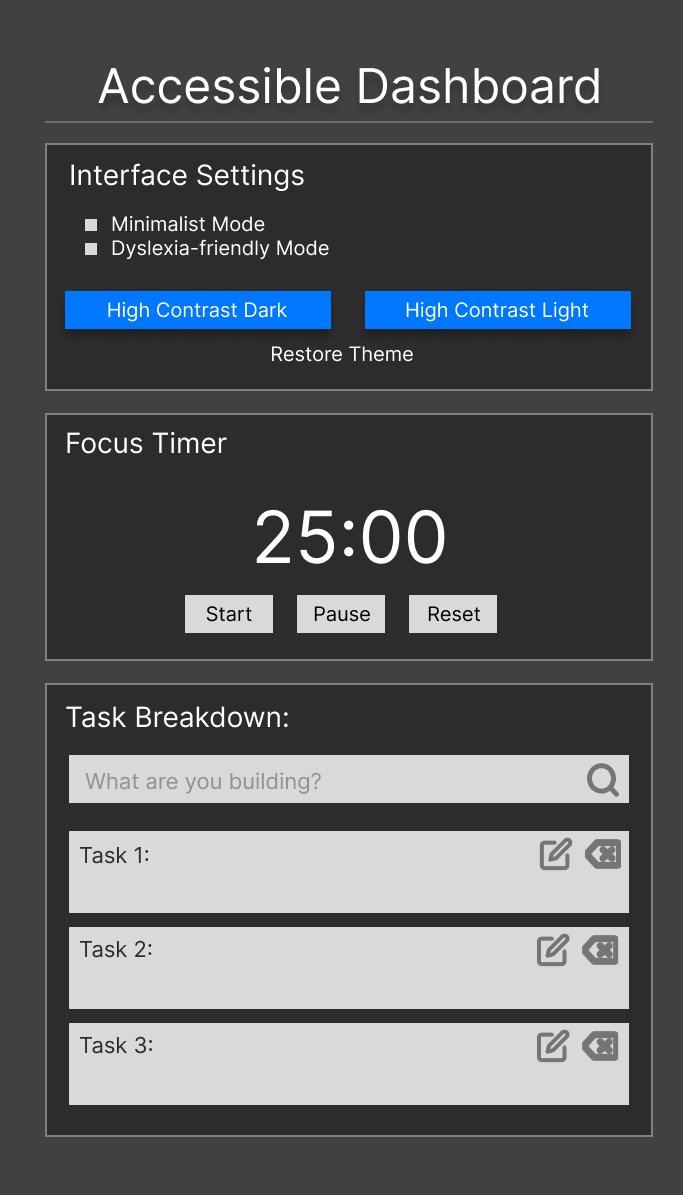
\includegraphics[width=0.6\linewidth, alt={}] {logos/Plug-in plan.png}
    \caption{UI Plan For the Accessible \gls{IDE} Plugin.}\label{fig:plug-inplan}
\end{figure}

THe first draft if the \gls{UI} was designed in figma, which allowed me get a clear vision of how the plugin would look and function. 
This also guaranteed that the design of the plugin was in line with the requirements that had been set out in the previous section.
Before having an a visual idea for the UI the plan was to implement it using HTML and CSS in a Webview, which allowed me to create a custom dashboard 
that could be easily accessed from within VS Code.

\subsection{Technology Stack}
The development of the plugin utilises a modern web-based stack compatible with the VS Code extension ecosystem to ensure high performance and seamless \gls{API} integration.
\begin{itemize}
    \item JavaScript: The primary programming language used for both the extension backend and the Webview frontend. It was chosen for its native compatibility with Node.js and its ability to handle asynchronous message passing between the UI and the extension host.
    \item Node.js: Acts as the runtime environment for the extension, providing the necessary \gls{API}s for file system access, process management, and the execution of imperative commands within the \gls{IDE}.
    \item VS Code Extension \gls{API}: The core framework used to manipulate the \gls{IDE} environment. Specifically, it facilitates interaction with workspace.getConfiguration for visual styling and vscode.commands for interface simplification.
    \item OpenAI \gls{API} / VS Code Language Model \gls{API}: Provides the generative intelligence required for the Task Architect and Code Explainer. By utilising the resident gpt-4o model, the plugin performs complex Chain of Thought~(\gls{CoT}) reasoning without requiring the user to provide personal \gls{API} keys.
    \item HTML/CSS: Used within the Webview layer to construct the Accessible Dashboard. This allows for the implementation of custom high-contrast themes and dynamic scaling that exceeds the limitations of standard VS Code CSS.
\end{itemize}

In terms of plugin development, the two main languages that are used
 are JavaScript and TypeScript. Although Typescript is more useful if the project was larger, I felt that JavaScript would be sufficient for the scope of this project and would 
 allow me develop the plugin quickly, especially due to the fast turn around time of the project. JavaScript was also chosen for its native compatibility with the VS Code 
 extension host and its ability to handle asynchronous message passing between the UI and backend.~\cite{TypeScri5:online}
 
For the \gls{AI} features, I decided to use the \textit{gpt-4o} model through the VS Code Language Model \gls{API}, which allows me to leverage powerful language models without 
requiring users to manage their own \gls{API} keys. Finally, I chose HTML and CSS for the Webview UI to allow for maximum flexibility in designing the dashboard 
and implementing custom themes. 

\subsubsection{Minimalist Toggle (FR1)}

The Minimalist Toggle serves as a reset for the \gls{IDE}. It utilises a state-management system to track the current visibility of the VS Code workbench.
When activated, it dispatches a batch of imperative commands to the vscode.commands \gls{API}, hiding the Activity Bar, Status Bar, Side Bar, and Breadcrumbs simultaneously.
By reducing the total number of visual elements on the screen, the module lowers extraneous cognitive load, allowing the developer to allocate more mental energy to the
code editor itself.


\subsubsection{Task Architect - \gls{AI}-Driven \Gls{scaffolding} (FR2)}
The Task Architect is a Human-in-the-Loop~(\gls{HITL}) module that facilitates \gls{task_initiation} by breaking down overwhelming objectives into granular steps. The module should employs 
a \gls{CoT} prompting strategy to take a complex task and break it down into simpler sub-tasks.
The generated steps are rendered as editable fields within the dashboard, allowing users to modify or refine the \gls{AI}'s suggestions. This ensures that developers 
maintain agency over their project architecture while the \gls{AI} handles the initial decomposition.
\newline

\textbf{Overcoming Latency and Verbosity}
\newline
During the testing of various prompt structures, a recurring challenge emerged, how much unnecessary text was included in the \gls{LLM}'s output.
 When asked to assist, the model frequently included excessive supportive dialogue. While intended to be user-friendly, this extra text hindered the system's 
 ability to parse the output into discrete, editable UI components.

To solve this issue, the prompt was refined to enforce a strict structural output, prioritising data over dialogue. This ensured that the generated steps 
could be seamlessly rendered as editable fields within the dashboard, preserving the developer's agency to modify or refine the architecture without sifting 
through conversational filler.


\textbf{Balancing Granularity and Utility}
\newline
Initial experiments with simple prompts such as ``How to code a login page'', the \gls{LLM} would bypass the architectural phase and provide a block of code immediately. 
This was counterproductive for two reasons:

\begin{itemize}
    \item It failed to provide a conceptual roadmap for the user.
    \item It increased the technical hallucination risk by attempting to solve a high-level task in a single step rather than planning the logic first.
\end{itemize}

\textbf{Increased Steps}
\newline
The original design specifications for the Task Architect called for 3 to 5 broad sub-tasks. However, user testing revealed that this flat structure remained overwhelming. A single step like ``Set up the backend'' was still too abstract for many users to execute confidently.
To address this, I implemented a hierarchical decomposition strategy. The system is now instructed to generate a primary set of sub-tasks, but with a critical addition: each sub-task must include two distinct micro-steps.

\subsubsection{Visual Styler} 
The Visual Styler is a specialised UI/UX module designed to manage the \gls{IDE}`s aesthetic environment, specifically targeting the reduction of eye strain and sensory overwhelm. By prioritising visual ergonomics, the module ensures that the development environment remains inclusive for \gls{neurodivergent} users and those with visual impairments.

\textbf{Accessibility and \gls{WCAG} Mapping}
\newline
To ensure the platform is accessible to the widest possible audience, the Visual Styler utilises a systematic mapping of presets based on the Web Content Accessibility Guidelines (WCAG) 2.1 Level AA.
\begin{itemize}
    \item High Contrast Modes: The module provides dedicated \textit{High Contrast Dark} and \textit{High Contrast Light} themes. These presets are programmatically validated to ensure a minimum contrast ratio of 4.5:1 for standard text and 3:1 for large text or UI components.
    \item Sensitivity Accommodations: By offering these specific color profiles, the \gls{IDE} addresses the needs of users with color vision deficiencies~(\gls{CVD}) and photophobia 
    (light sensitivity), allowing for a high-degree of legibility without triggering sensory fatigue.
\end{itemize}

\textbf{Technical Implementation and Functionality}
\newline
The Visual Styler operates by interacting directly with the workspace.getConfiguration \gls{API}. This allows the module to move beyond surface-level CSS changes and manipulate the core structural rendering of the workspace:

Dynamic Scaling: Users can adjust font sizes and line heights across the entire interface. Increasing the line height (e.g., to 1.5 or 2.0) is a critical intervention for developers with \gls{dyslexia}, as it reduces the crowding effect of text and improves character recognition.

Granular Customisation: Unlike traditional static themes, the Styler follows a visual comfort framework. It treats font-weight, letter spacing, and padding as variables that the user can tune to their specific cognitive load requirements.

User Agency and Sensory Regulation
By providing an intuitive dashboard for these adjustments, the Visual Styler empowers the developer to curate their own sensory environment. This reduces the cognitive energy spent on deciphering a cluttered or poorly-lit UI, allowing that energy to be redirected toward the primary task of programming. The module essentially acts as a sensory filter, ensuring that the \gls{IDE} adapts to the user`s biological needs rather than forcing the user to adapt to a rigid interface.

\subsection{System Architecture}
The system is divided into three primary layers: the Presentation Layer (Webview), the Orchestration Layer (Extension Host), and the External Services Layer (VS Code \gls{API}).

1. The Presentation Layer: WebView UI

The user interface is implemented as a \texttt{WebviewPanel}, which renders a custom HTML/JavaScript dashboard. This allows for a highly flexible UI where the extension to be customised to best fit the user's needs, predetermined through prior research.

\begin{itemize}
    \item State Communication: Because WebViews are isolated from the main editor, communication is handled via asynchronous message passing. The UI dispatches JSON-formatted messages using \texttt{vscode.postMessage()}, which are then intercepted by the extension’s backend.
    \item Asynchronous Feedback: The UI remains responsive by using event listeners that wait for \texttt{updateTime}, \texttt{taskResult}, or \texttt{errorResult} commands sent back from the extension host.
\end{itemize}

2. The Orchestration Layer: Extension Host

The core logic resides in the activate function, which serves as the central hub while the extension is active.

\begin{itemize}
    \item Command Registration: The system registers specific URI commands (e.g., accessible-toggle.showUI) that map user intents to internal JavaScript functions.
    \item Configuration Management: A key architectural feature is the interaction with getConfiguration. The extension reads and writes global settings to modify the editor's environment (font size, themes, and layout) in real-time, effectively acting as a wrapper for the VS Code Settings engine. 
    \item Context Preservation: To ensure the system is non-destructive, the architecture utilises \texttt{context.globalState}. This allows the extension to store the user`s original theme and font settings before applying accessibility modifications, enabling a seamless restoration process. This also acts as a form of error prevention in case any settings are applied by accident.
\end{itemize}


3. The Functional Providers

The architecture employs specialised logic blocks to handle distinct accessibility needs:

\begin{table}[ht]
    \centering
    \caption{System Component Interaction and \gls{API} Dependencies}\label{tab:system_architecture}
    \small % Slightly smaller text to ensure it fits the margins
    \begin{tabular}{@{} l p{4cm} l @{}}
        \toprule
        \textbf{Component} & \textbf{Interaction Strategy} & \textbf{VS Code API Dependency} \\ 
        \midrule
        Interface Controller & Imperative Commands          & \texttt{commands.executeCommand} \\
        Theme/Font Engine    & Configuration Updates        & \texttt{workspace.getConfiguration} \\
        Task Architect       & \gls{AI} Stream Processing         & \texttt{vscode.lm} (Language Model) \\
        Code Helper          & Diagnostic Polling           & \texttt{languages.getDiagnostics} \\
        \bottomrule
    \end{tabular}
\end{table}

4. Integration with Language Models 

The \textit{Task Architect} and \textit{Code Helper} features utilise the VS Code Language Model \gls{API}. This architectural choice ensures security and efficiency, as the extension does not require individual \gls{API} keys from the user. Instead, it requests access to the editor's resident models (e.g., GPT-4o). The system uses a \gls{CoT} prompting strategy to process raw diagnostic data or user goals into structured, \gls{neurodiverse}-friendly steps before pushing the data back to the Presentation Layer.


\subsection{UI Simplification and Minimalist Toggle (FR1)}
The implementation of the Minimalist Mode focuses on reducing visual noise, which research identifies as a primary driver of cognitive overload and sensory overwhelm for autistic and \gls{ADHD} developers.
 This module acts as a digital ramp, filtering environmental noise to prevent the exhaustion of a developer's limited cognitive budget.
 
 The technical execution follows an imperative command pattern to provide a seamless, one-click transition:
\begin{itemize}
 \item \textbf{Workspace Manipulation:} Using the vscode.commands.executeCommand \gls{API}, the plugin simultaneously toggles the visibility of the Activity Bar, Side Bar, Status Bar, and Breadcrumbs.
 \item \textbf{Global Configuration:} To remove persistent distractions like the Mini-map, the system interacts directly with global user settings using config.update('editor.minimap.enabled', ...).
 \item \textbf{State Management:} The module utilises a state-management system to track the current visibility of the VS Code workbench.
 \item \textbf{Non-Destructive Restoration:} To mitigate anxiety regarding lost settings, the architecture employs context.globalState to store the original UI configuration. This allows users to revert all changes instantly, satisfying the requirement for a safe and reversible interface.
 \end{itemize}

 By centralising these actions into a single toggle, the plugin lowers Extraneous Cognitive Load (\gls{EL}). This allows the developer to reallocate mental resources from navigating a complex, high-density interface toward \gls{GL}, the actual logical problem-solving and programming tasks

\textbf{Final UI/Functionality Integration (FR1)}
\begin{figure}[H]
    \centering
    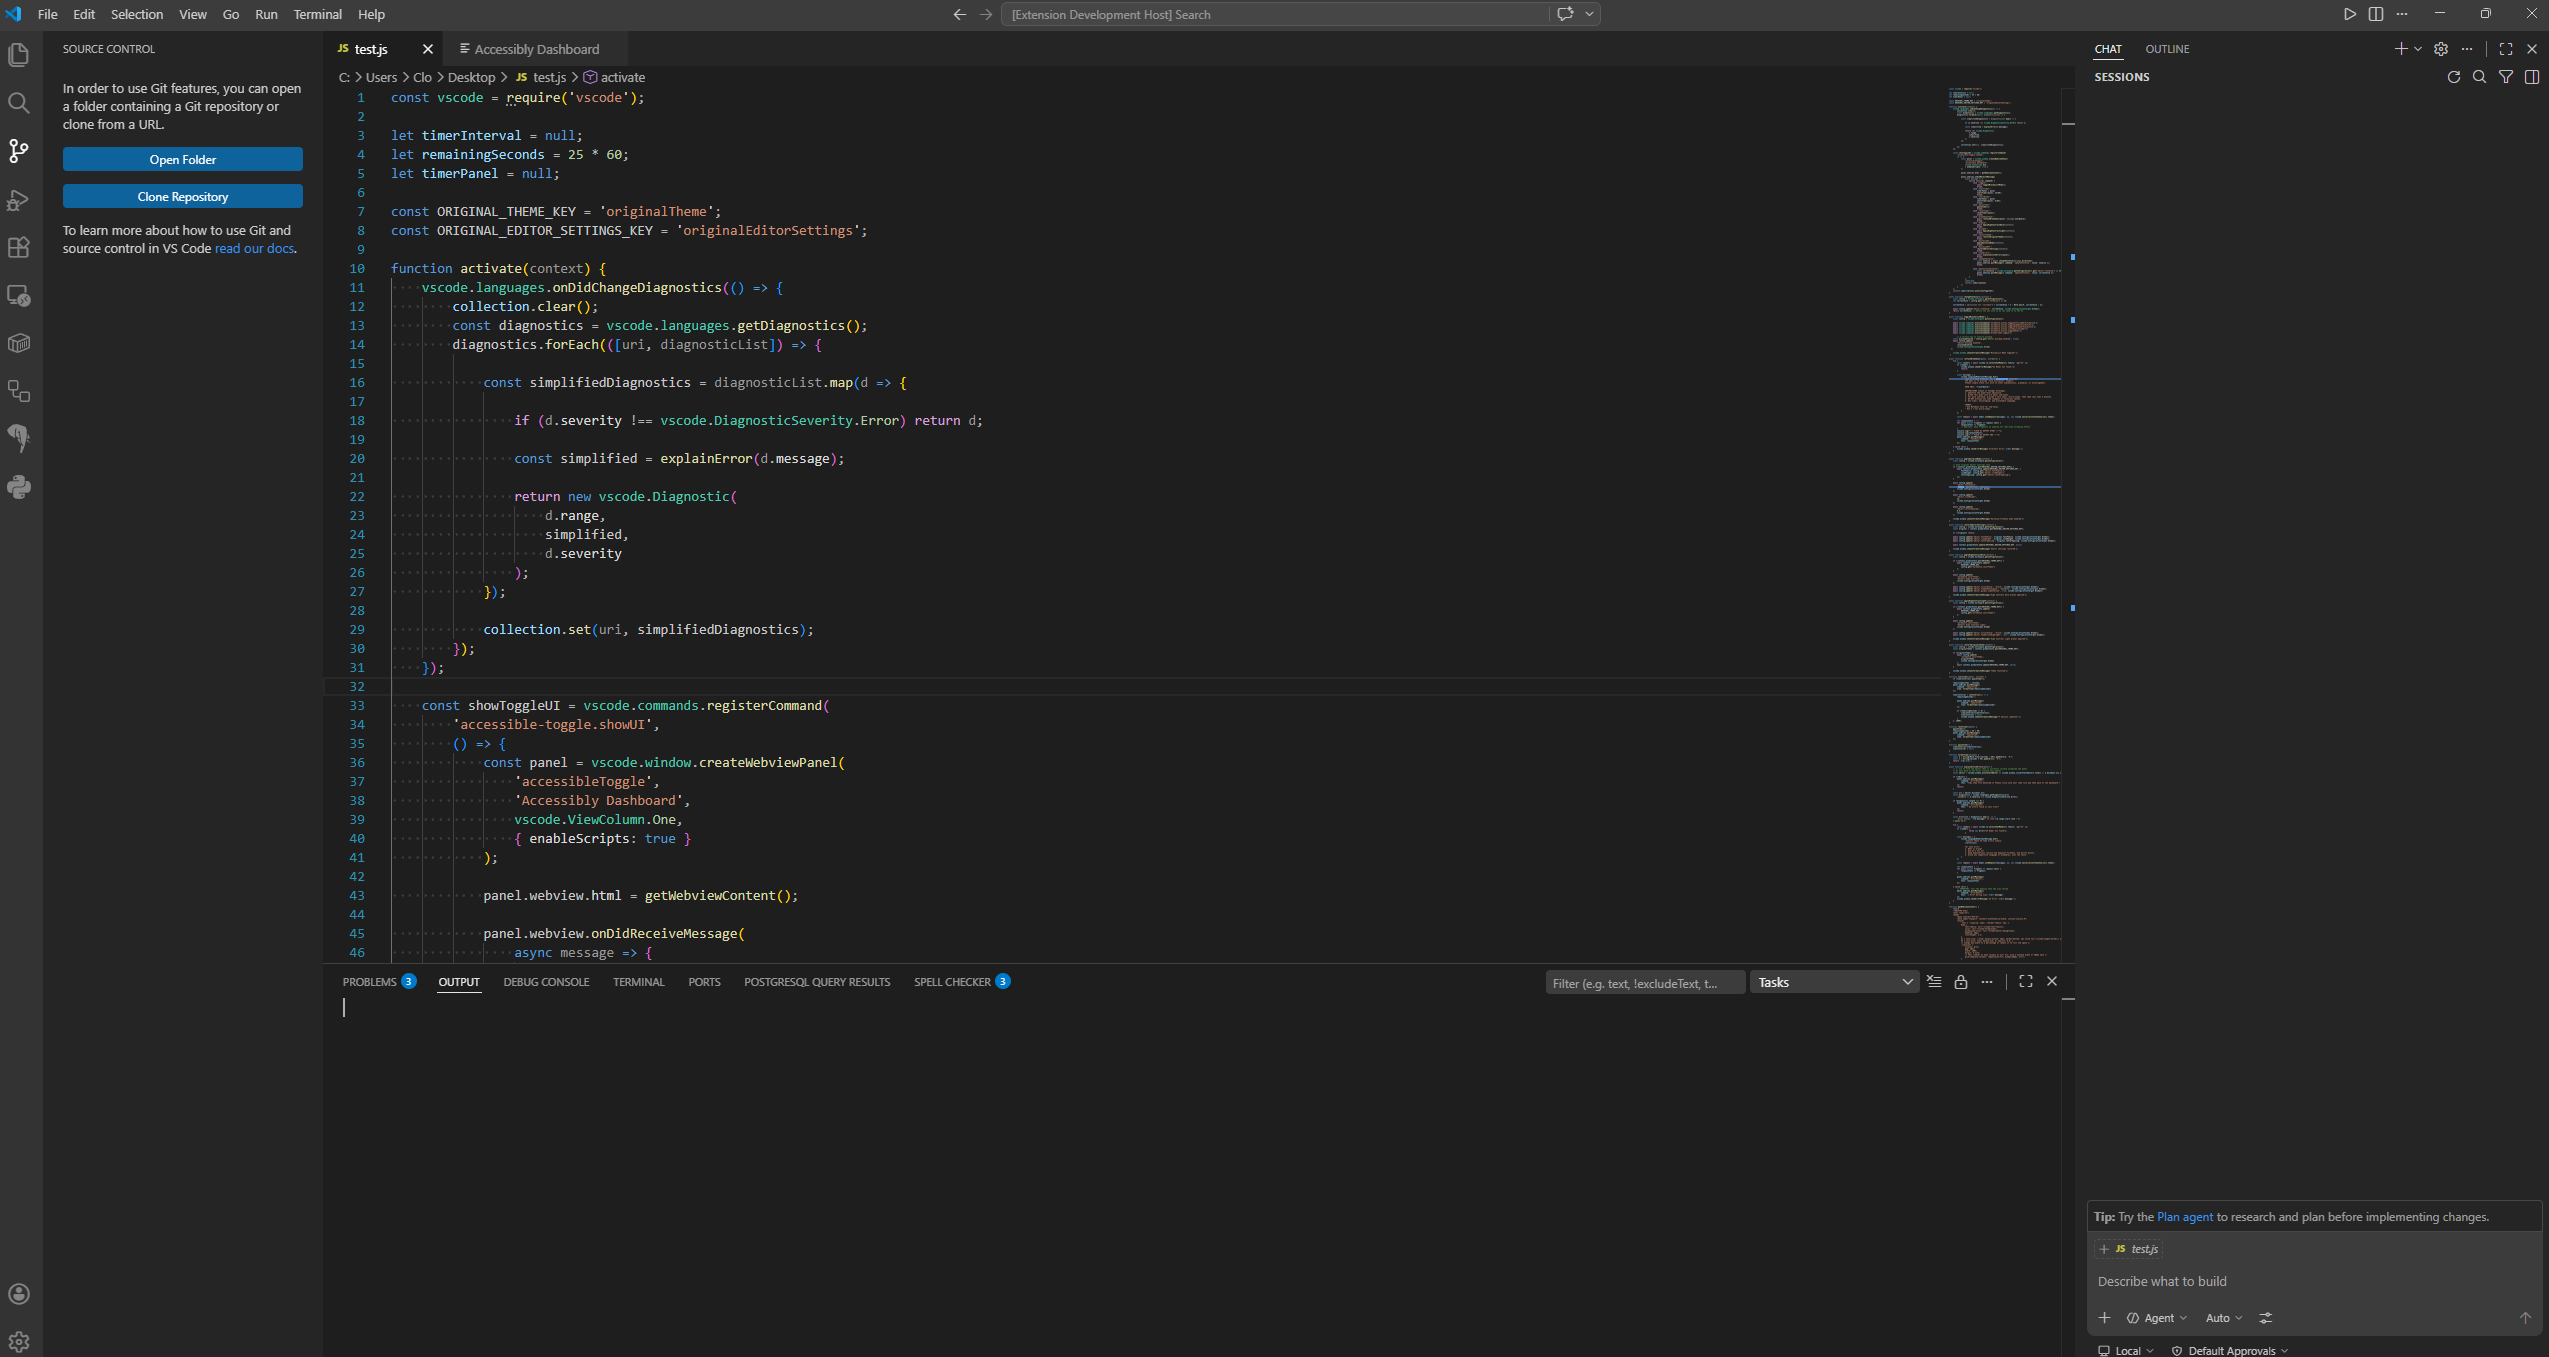
\includegraphics[width=0.9\linewidth, alt={}] {logos/preMinimal.png}
    \caption{Pre-Minimalist UI, showing the default VS Code interface with all standard elements visible.}\label{fig:PreMinimal}
\end{figure}

\begin{figure}[H]
    \centering
    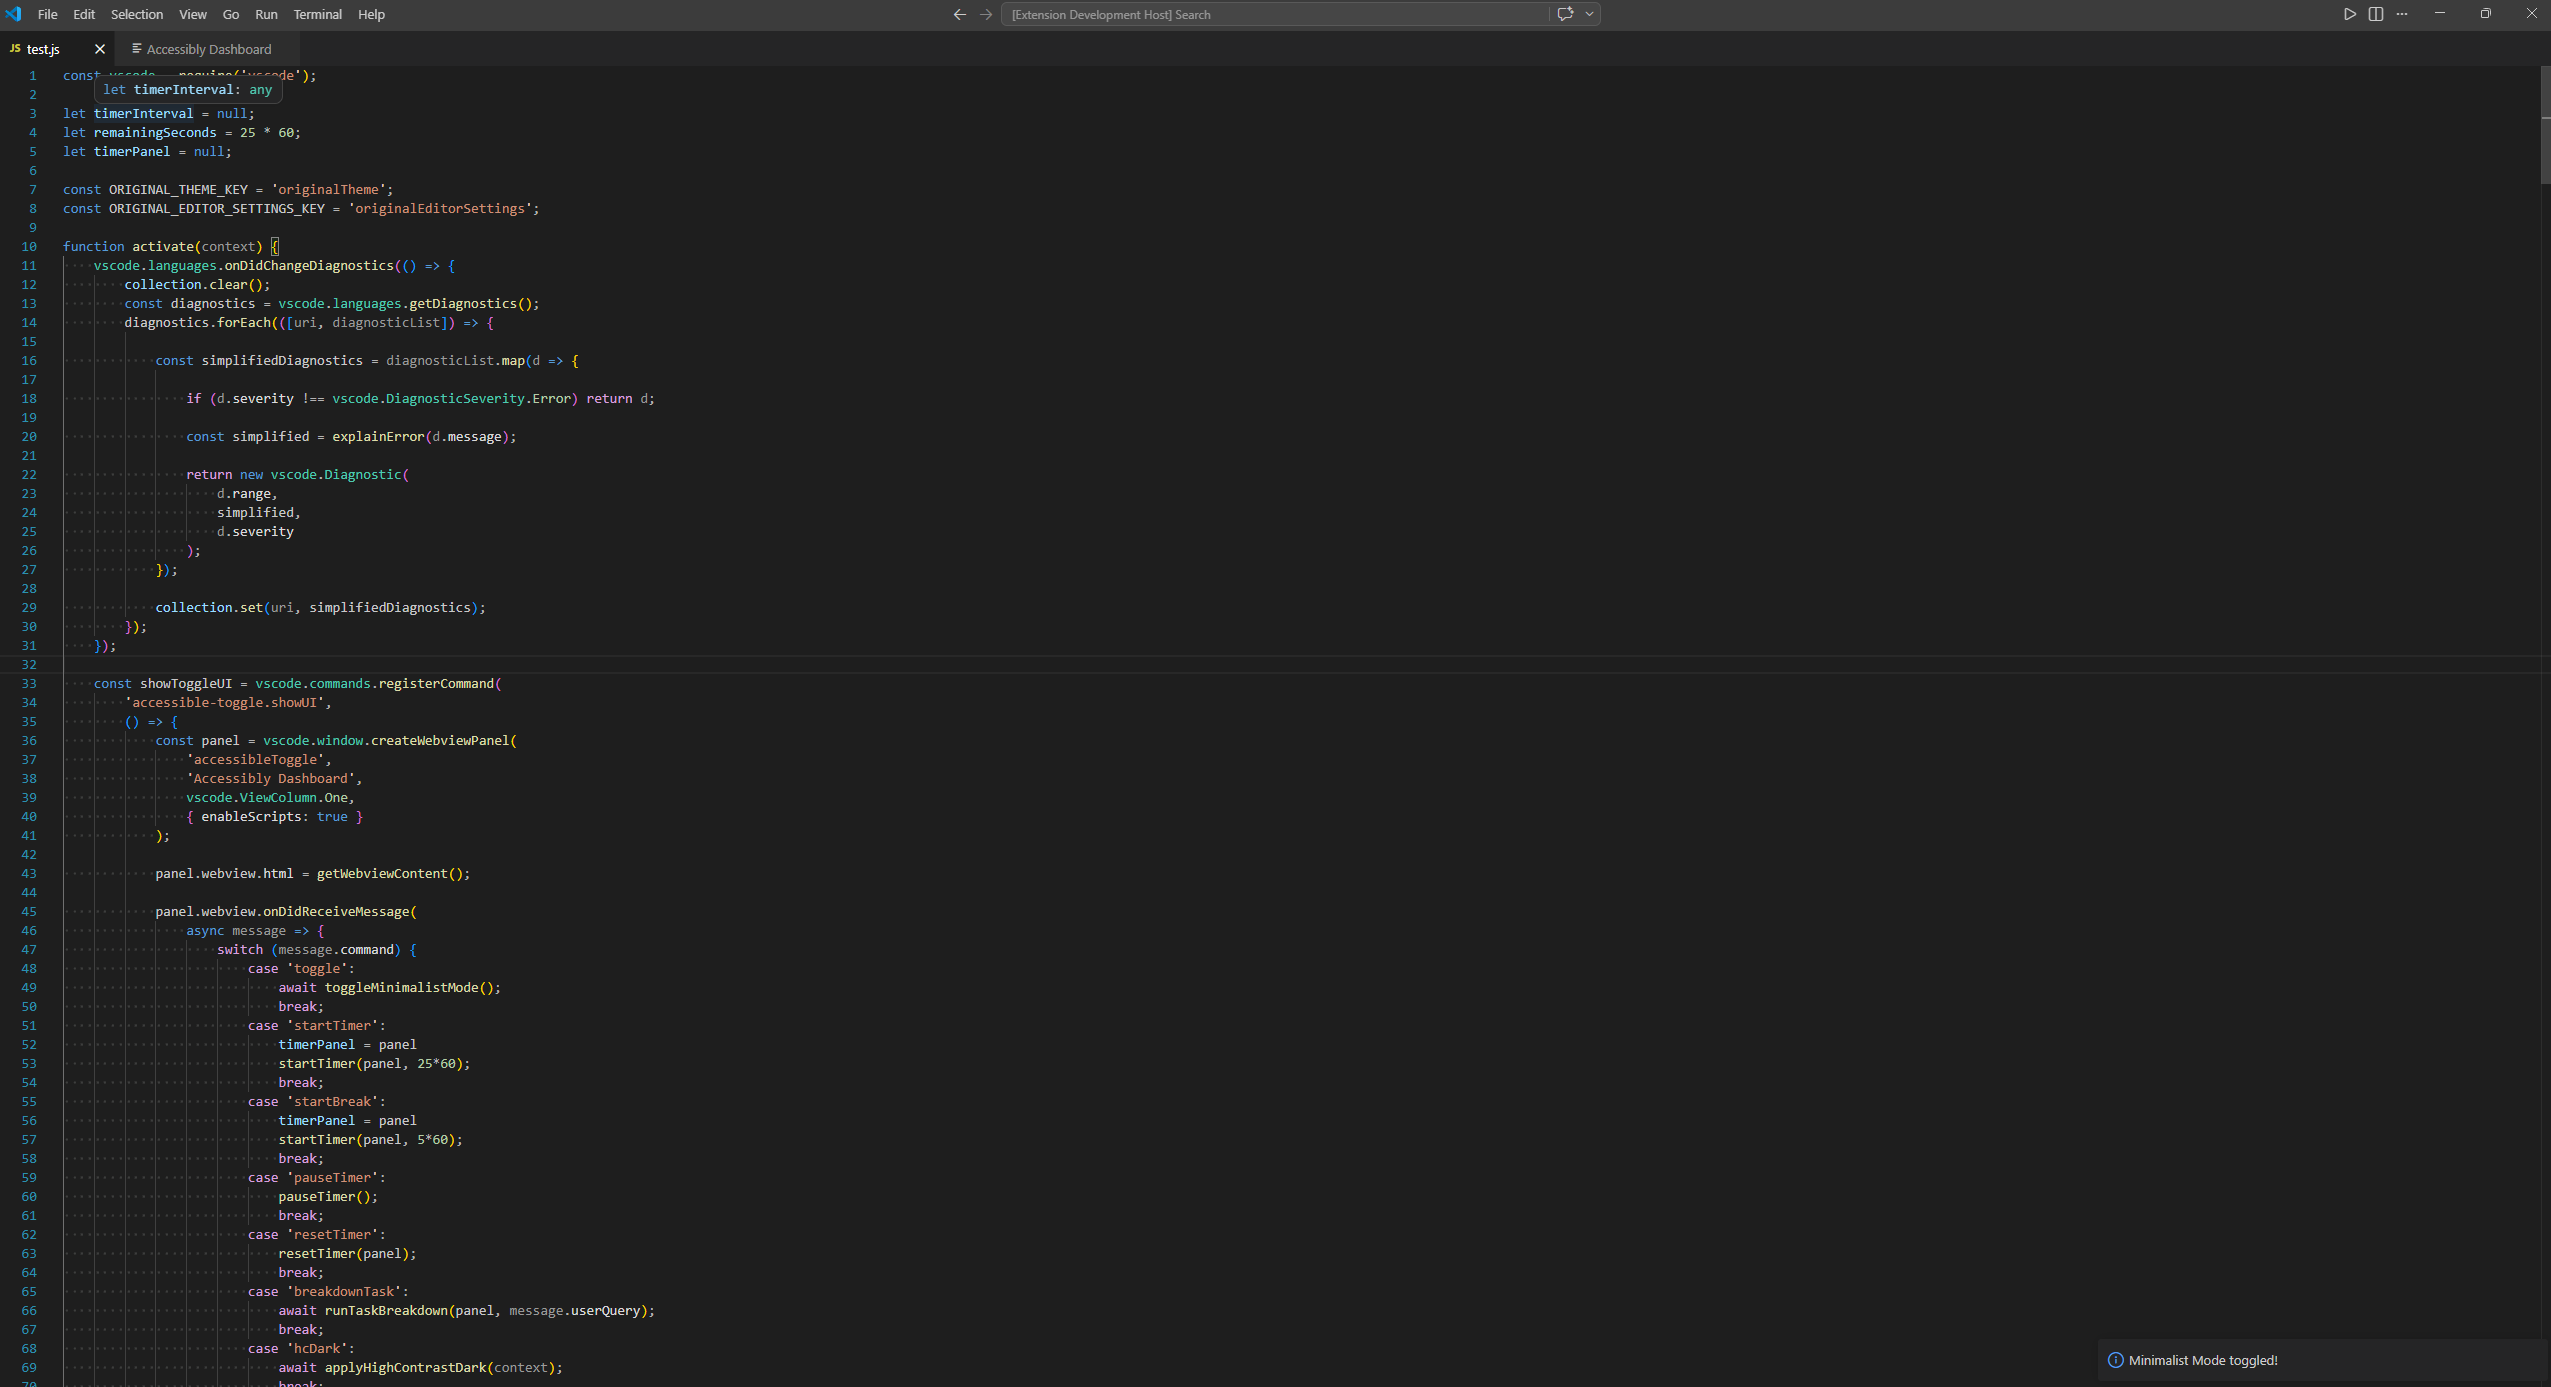
\includegraphics[width=0.9\linewidth, alt={}] {logos/postMinimal.png}
    \caption{Post-Minimalist UI, showing the simplified VS Code interface with reduced visual elements.}\label{fig:PostMinimal}
\end{figure}

\begin{figure}[H]
    \centering
    
\includegraphics[width=0.7\linewidth, alt={}] {logos/MinimalNote.png}
    \caption{Notification confirming the activation of Minimalist Mode, providing immediate feedback to the user.}\label{fig:MinimalNote}
\end{figure}

\subsection{\gls{AI} Integration (FR2 and FR3)}
The \gls{AI}-driven features are implemented using a Streaming Data Pattern to satisfy NFR3 (Latency), ensuring the interface remains responsive during complex generation.

\subsubsection{Task Architect: Overcoming \Gls{task_paralysis}}
\begin{itemize}
\item \textbf{Prompt Engineering:} The \textit{Task Architect} uses a strictly defined system prompt to enforce a micro-step structure (3--5 sub-tasks with two 5-minute 
micro-steps each). This prevents the \gls{LLM} from generating a long response that can be overwhelming.
\item \textbf{Iterative Prompt Refinement:} During development, I identified a significant limitation where the \gls{LLM} included excessive supportive dialogue 
(e.g., ``Sure! I can help with that''). While polite, this violated the principle of Direct Instruction and hindered the system's ability to parse the text into 
editable UI components. I refined the prompt to mandate a strict data-only format, ensuring the system only outputs actionable tasks.
\end{itemize}

\begin{figure}[H]
    \centering
    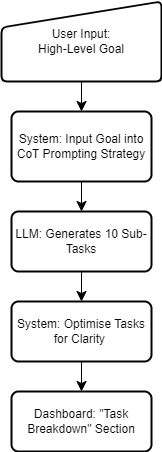
\includegraphics[width=0.3\linewidth, alt={}] {logos/aiflow.png}
    \caption{\gls{AI} Flow for the Task Architect Module.}\label{fig:AIflow}
\end{figure}

The Figure~\ref{fig:AIflow} demonstrates the process of the Task Architect module. When a user enters a high-level goal (e.g., ``Implement a search bar''), the system 
instructs the \gls{LLM} to output 3-5 actionable sub-tasks with 2 additional tasks from each of the sub-tasks.
 
\begin{figure}[H]
    \centering
    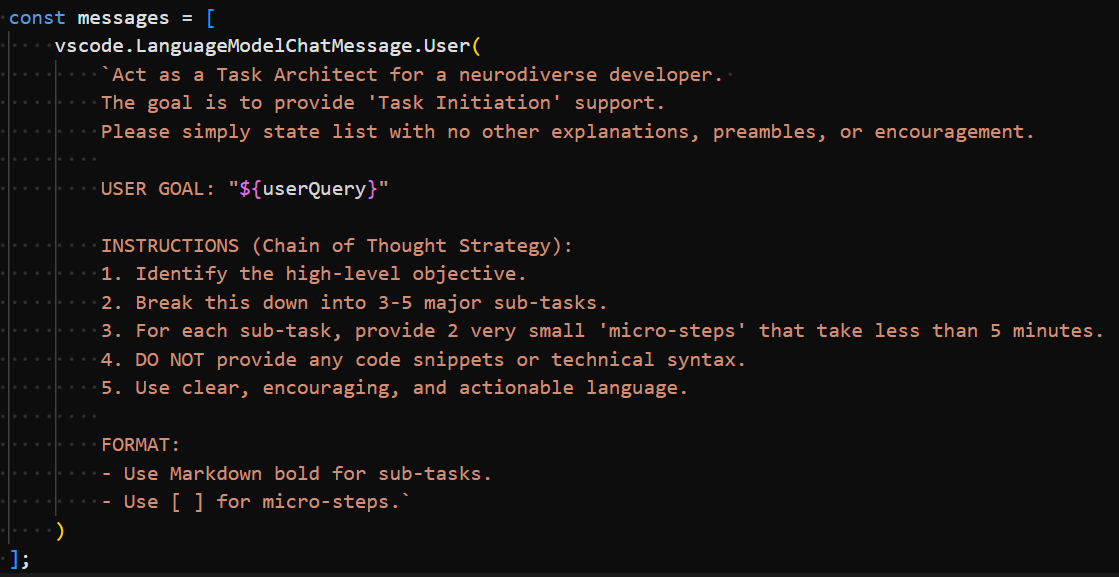
\includegraphics[width=1\linewidth, alt={}] {logos/aicode.png}
    \caption{Code written to generate tasks}\label{fig:AIcode}
\end{figure}

Not only does the this prompt ask the \gls{LLM} to break down the task, but it also instructs it to format the output in a specific way.
So that the response can be easily broken down and cleaned for the output the prompt includes instructions to make sure the subtasks in bold and the micro-steps are preceded by ``[ ]''.

\subsubsection{Human-in-the-Loop (HITL) Implementation}
As shown in Figures~\ref{fig:taskoutput} and~\ref{fig:taskarchitect}, the generated tasks are rendered in the dashboard as editable fields. This is a critical design choice to preserve User Agency. 
\Gls{neurodivergent} developers often have unique workflows so by allowing the user to edit or delete \gls{AI}-generated steps, the tool moves from being a prescriptive authority 
to a flexible partner. The graying-out of completed tasks provides immediate visual feedback, supporting \gls{working_memory} by externalising task progress.

\begin{figure}[H]
    \centering
    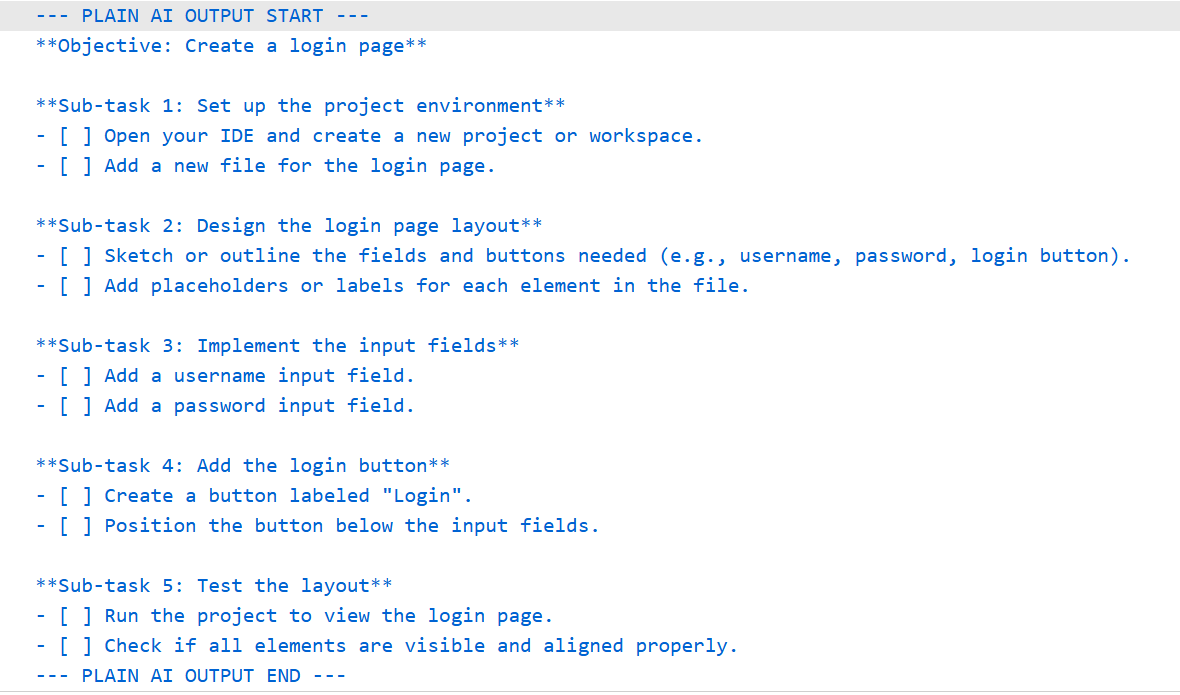
\includegraphics[width=0.8\linewidth, alt={}] {logos/taskoutput.png}
    \caption{Example of the output generated by the Task Architect module, showing the micro-steps for a given task.}\label{fig:taskoutput}
\end{figure}

\begin{figure}[H]
    \centering
    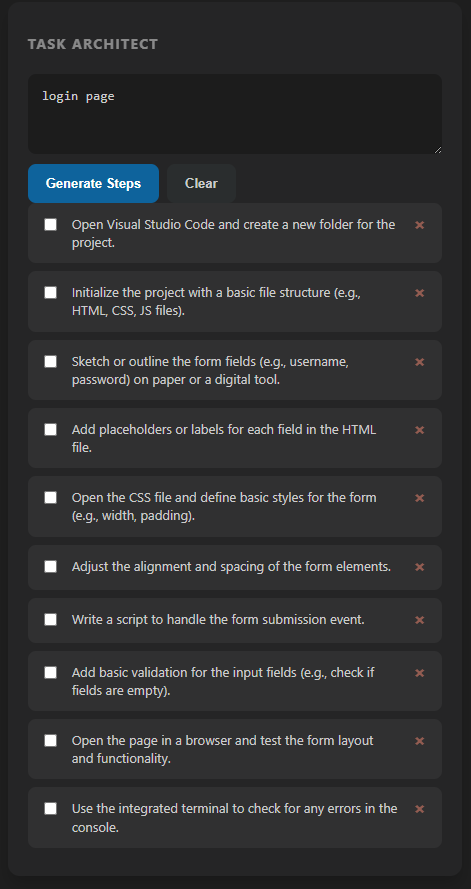
\includegraphics[width=0.6\linewidth, alt={}] {logos/taskarchitect.png}
    \caption{Task Architect Module in the Dashboard, showing the generated tasks.}\label{fig:taskarchitect}
\end{figure}

\subsubsection{Code Explainer: Mitigating Technical Cognitive Overload}
The Code Explainer is a diagnostic interceptor designed to address the high extraneous cognitive load often imposed by cryptic compiler errors. 
For neurodivergent developers, particularly those with \gls{ASD}, standard diagnostic messages can be ambiguous, leading to a breakdown in task 
momentum.

\textbf{Technical Implementation and Workflow}


The module is implemented as an asynchronous function, explainActiveErrors, which operates through a three-stage pipeline: Detection, Extraction, and Translation.
\begin{itemize}
    \item Detection: The system first verifies that a code file is active within the editor. If no file is detected, the system provides a clear, actionable 
instruction to the user: "No code file detected. Please click into your code file and then back to the dashboard." This ensures that the user understands 
the necessary context for the feature to function, reducing confusion and promoting a sense of control.
    \item Extraction: Using the vscode.languages.getDiagnostics \gls{API}, the module identifies active compiler issues. To minimise noise, 
    the system specifically filters for vscode.DiagnosticSeverity.Error, ensuring the developer is not overwhelmed by warnings or information-level 
    messages that do not immediately block execution.
    \item Translation: The raw error messages and their corresponding line numbers are compiled into an errorList string. 
This list is then dispatched to the resident \textit{gpt-4o} model via the VS Code Language Model \gls{API}.
\end{itemize}

\textbf{Prompt Engineering for Direct Instruction}


To satisfy the requirement for beginner-friendly, non-technical feedback, the module employs a strictly constrained system prompt. The \gls{AI} is instructed to:
\begin{itemize}
    \item Identify the problem and provide a specific fix.
    \item Maintain a concise, bulleted format.
    \item Avoid all \textit{supportive language} or conversational preambles.
\end{itemize}

This approach aligns with the principle of Direct Instruction, reducing the \gls{cognitive_tax} required to 
filter through polite but unnecessary conversational filler.

\subsection{\Gls{dyslexia} Settings: Test spacing (FR5)}
The Visual Styler module allows users to adjust the spacing between characters and line height in the \gls{IDE}. This is particularly beneficial for developers with \gls{dyslexia}, as increasing letter spacing 
and vertical padding can significantly reduce the crowding effect in dense code, improving character recognition and overall readability. 

    To balance customisability with cognitive ease, the plugin provides a set of predefined spacing presets, \textit{Standard, Relaxed, and Spacious},
for the users to choose from in the dashboard. This allows for quick adjustments without overwhelming the user with too many options, while still providing the 
necessary customisation to accommodate different cognitive needs.

The presets implement a hierarchical increase in visual breathing room:
\begin{itemize}
    \item Standard: Acts as a soft reset to default editor settings ($lineHeight: 0$, $letterSpacing: 0$) using the system's standard font family.
    \item Relaxed: Increases the $lineHeight$ to $30$ and $letterSpacing$ to $0.8$, introducing specialised fonts such as Lexend and OpenDyslexic.
    \item Spacious: Offers the maximum level of separation with a $lineHeight$ of $40$ and $letterSpacing$ of $1.5$. This preset prioritises OpenDyslexic as the primary font to further enhance character distinction.
\end{itemize}

The inclusion of OpenDyslexic and Lexend is a critical design choice; these fonts use 
weighted bottoms or unique shapes to help the brain distinguish between similar
characters (e.g., ``b'' vs ``d''), which is a common hurdle for dyslexic readers. 
By offering these as a unified \textit{Spacious} preset, the plugin provides a high-signal 
environment that accommodates diverse cognitive needs with minimal interaction cost.

\subsubsection{Initial Plan: One Option}
Initially, the plugin was programmed with fixed values for line height and letter spacing. 
However, user testing revealed that a one-size-fits-all approach was insufficient, as 
individual cognitive needs regarding text density vary significantly.

The figures below demonstrate the visual impact of these adjustments. 
Figure~\ref{fig:vanillasettings} displays the standard VS Code environment, 
while Figure~\ref{fig:dyslexiasettings} illustrates the enhanced readability achieved
 by increasing the line height to 1.5 and the letter spacing to 0.5em.

\begin{figure}[H]
    \centering
    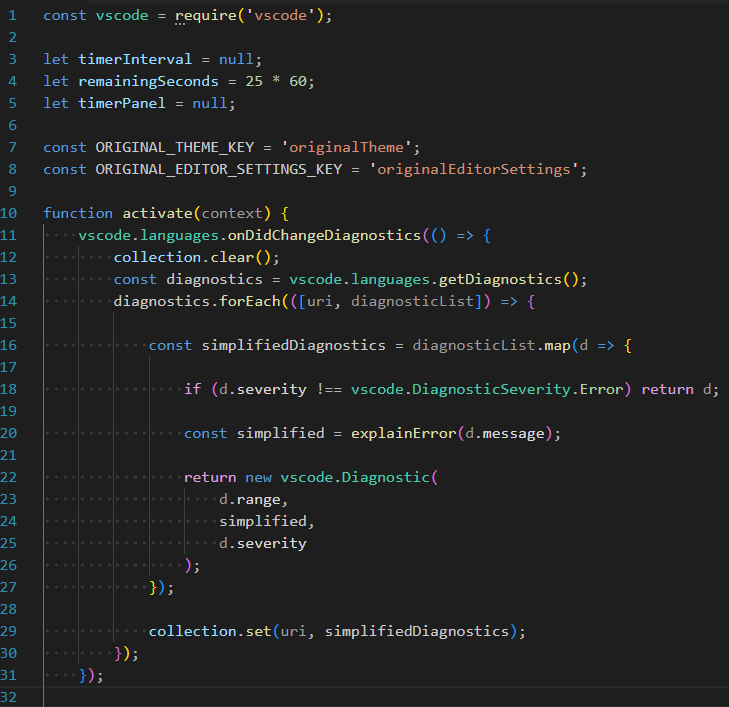
\includegraphics[width=0.7\linewidth, alt={}] {logos/van.png}
    \caption{Example of the difference in spacing between the default settings and the original \gls{dyslexia} settings, where the line height is set to 1.5 and the letter spacing is set to 0.5em.}\label{fig:vanillasettings}
\end{figure}

\begin{figure}[H]
    \centering
    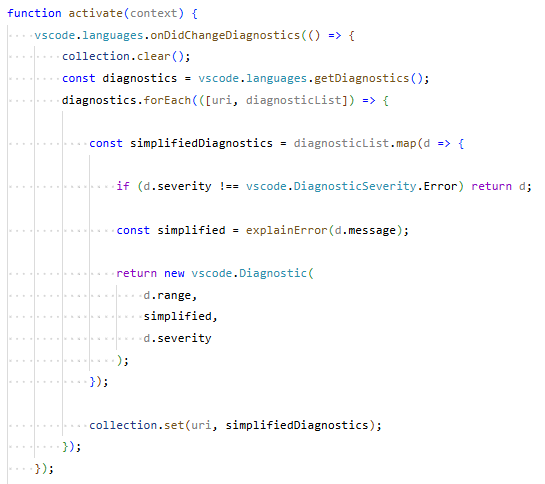
\includegraphics[width=0.7\linewidth, alt={}] {logos/bas.png}
    \caption{Example of the difference in spacing between the default settings and the original \gls{dyslexia} settings, where the line height is set to 1.5 and the letter spacing is set to 0.5em.}\label{fig:dyslexiasettings}
\end{figure}

\subsubsection{Final UI Integration}
The final UI design (see Figure~\ref{fig:dyslexiamenu}) unifies the Visual Styler with other cognitive aids to ensure that environment modification is non-destructive and instantaneous:
\begin{figure}[H]
    \centering
    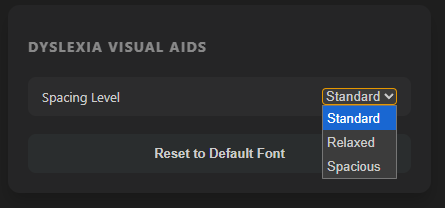
\includegraphics[width=0.7\linewidth, alt={}] {logos/dislecMenu.png}
    \caption{The UI implementation of the line spacing tool}\label{fig:dyslexiamenu}
\end{figure}
The evolution from fixed values to the hierarchical preset system (Standard, Relaxed, Spacious) 
represents a shift toward a user-centric sensory model. By centralising these 
complex font and spacing configurations into a single module within the 
Accessible Dashboard, the plugin minimises the executive tax required to curate
a readable workspace.

\begin{itemize}
    \item One-Click Presets: Instead of navigating nested VS Code menus, users select the \textit{Dyslexia-friendly Mode} or specific high-contrast buttons. This reduces interaction depth from approximately six clicks to one, significantly lowering extraneous cognitive load.
    \item Immediate Visual Confirmation: The dashboard provides real-time feedback, eliminating the verification anxiety common when \gls{neurodivergent} users must exit menus to see if changes were applied.
    \item Typography Hierarchy: The final implementation ensures that selecting a preset like \textit{Spacious} simultaneously updates three variables: increasing $lineHeight$ to 40, $letterSpacing$ to 1.5, and switching the typeface to OpenDyslexic.
    \item Non-Destructive Restoration: A critical component of the final UI is the \textit{Restore Theme} and reset functionality. This allows developers to experiment with spacing and contrast without the anxiety of losing their original, custom \gls{IDE} configurations.
\end{itemize}

\begin{figure}[H]
    \centering
    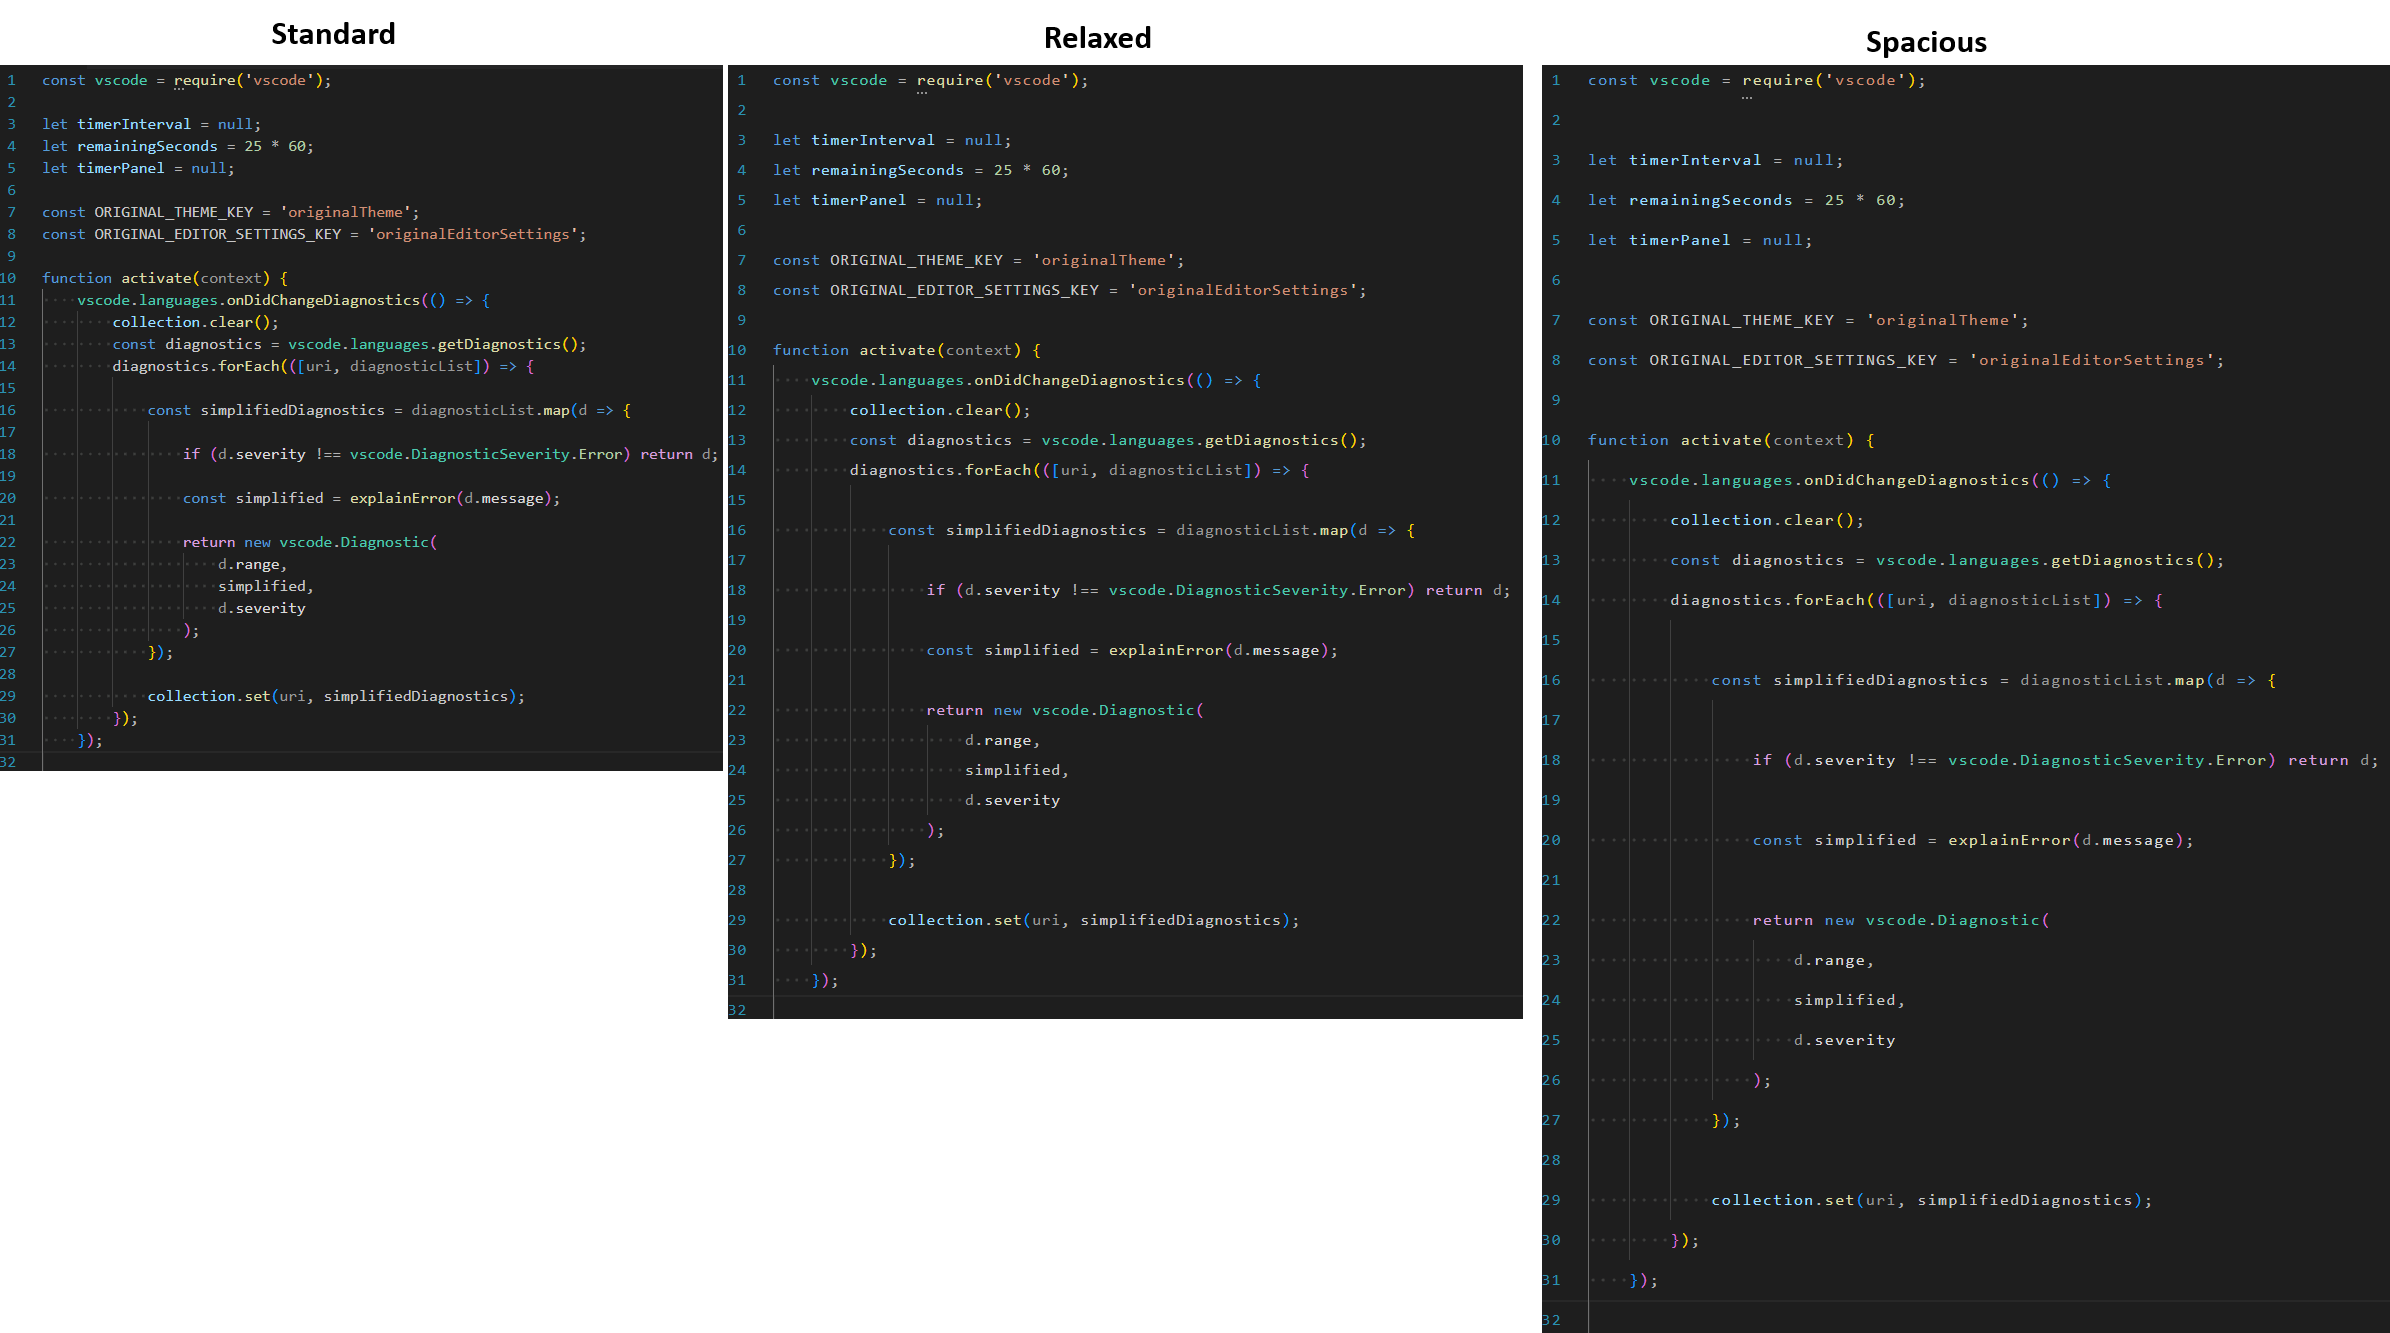
\includegraphics[width=1.6\linewidth, angle=90, alt={}] {logos/textOptions.png}
    \caption{Text spacing options implemented}\label{fig:dyslexiaText}
\end{figure}

\subsection{Pomodoro Timer (FR4)}
As mentioned in the literature review, the Pomodoro technique can be an effective tool for managing time and maintaining focus, especially for individuals with \gls{ADHD}. 
The plugin includes a customisable Pomodoro timer that allows users to set their own focus intervals and break durations. This flexibility is crucial, as a standard
 25-minute focus period may not be suitable for everyone.

The timer is integrated into the dashboard, providing a visual countdown and notifications when it's time to take a break or return to work. By allowing users to tailor 
the timing to their own rhythms, the plugin helps to reduce \glspl{state_recovery_cost} associated with interruptions and supports sustained focus.

\begin{figure}[H]
    \centering
    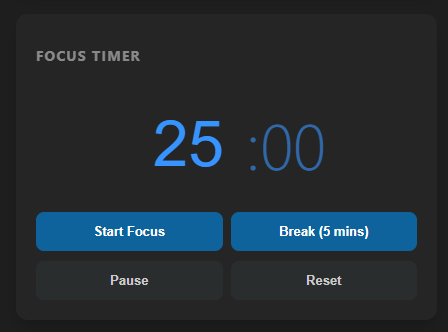
\includegraphics[width=0.6\linewidth, alt={}] {logos/timerFinal.png}
    \caption{Final design of the Pomodoro timer. The timer is directly editable, allowing users to set their own focus and break durations.}
    \label{fig:TimerFinal}
\end{figure}

\subsection{Initial User Testing and Feedback}
Initial user testing focused on the plugin's usability and functionality, revealing three critical areas for improvement. These are: 
UI clarity, \gls{AI} reliability, and efficiency. Feedback indicated that original labels like ``Decompose'' were too abstract, 
leading to a redesign of the Task Architect with clearer button labeling (``Generate Steps'') and contextual placeholders.
\begin{figure}[H]
    \centering
    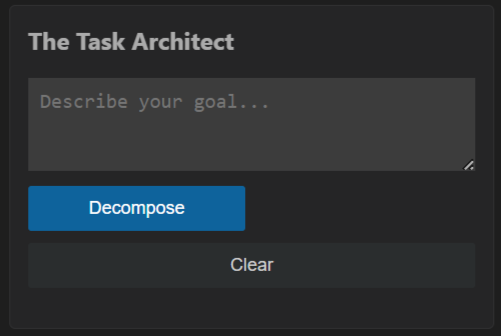
\includegraphics[width=0.6\linewidth, alt={}] {logos/uiprefix1.png}
    \caption{UI at the time of initial user testing, before improvements to the UI and \gls{AI} response integrity were made.}\label{fig:uiprefix}
\end{figure}

\begin{figure}[H]
    \centering
    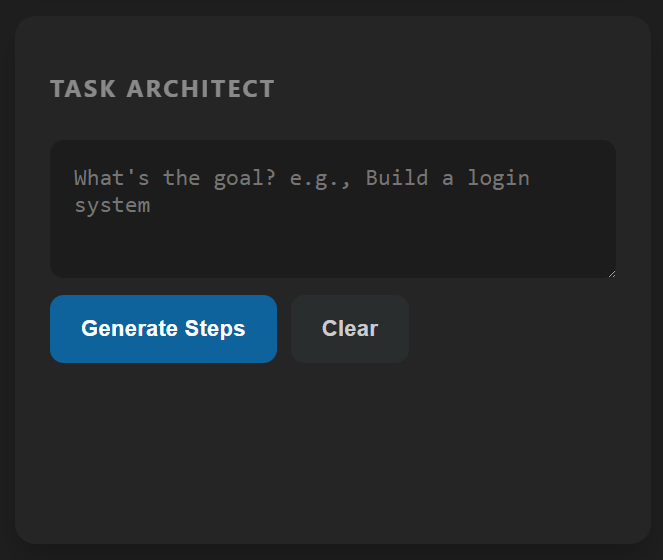
\includegraphics[width=0.6\linewidth, alt={}] {logos/uipostfix1.png}
    \caption{UI after improvements to the UI and \gls{AI} response integrity were made.}\label{fig:uipostfix}
\end{figure}


Technical evaluations also identified a parsing bug that truncated \gls{AI} responses, which was resolved by implementing a robust 
regular expression strategy to ensure full rendering of micro-steps. Finally, comparative testing against standard VS 
Code demonstrated the plugin's ability to significantly reduce cognitive load; specifically, the user performed accessibility 
adjustments,such as theme switching, in just 1.9 seconds (one click) compared to 19.9 seconds (six clicks) in the standard \gls{IDE}. 
These refinements ensured the tool successfully provided a more direct, inclusive path for \gls{task_initiation} and environment customisation.

\subsection{Final UI}
The final UI of the Accessibly Dashboard (see Figure~\ref{fig:finalui}) serves as the unified control center for the plugin`s assistive features. 
Designed as a centralised Webview panel, it provides a low-friction entry point that reduces the executive tax required to manage 
a complex development environment.

The interface is structured into modular sections to support inhibitory control and \gls{working_memory}:

\textbf{Interface Settings and Theme Presets}
\begin{itemize}
\item Minimalist Toggle: A single-click switch ("Close Panels") that simultaneously hides the Activity Bar, Side Bar, Status Bar, 
and Breadcrumbs to suppress Extraneous Cognitive Load.
\item Dyslexia Mode: A global toggle to quickly apply readability enhancements.
\item Soft High Contrast: Includes presets like "Soft HC Dark" and "Soft HC Light" to provide high signal without the sensory 
\gls{halation} risks of pure black-and-white themes.
\item Restore Original: A non-destructive reset button that supports psychological safety by allowing users to instantly 
revert all environmental changes.
\end{itemize}

\textbf{\Gls{dyslexia} Visual Aids and Text Scaling}
\begin{itemize}
\item Hierarchical Spacing: A dropdown menu offering Standard, Relaxed, and Spacious presets. Selecting \textit{Spacious} programmatically 
adjusts line height to 40, letter spacing to 1.5, and switches the font to OpenDyslexic.
\item Granular Scaling: A dedicated text scaling module allows users to tune the font size in real-time, providing immediate visual 
confirmation and eliminating verification anxiety.
\end{itemize}

\textbf{AI-Driven \Gls{scaffolding}}
\begin{itemize}
    \item Task Architect: A Human-in-the-Loop (HITL) module where users input high-level goals. The \gls{AI} decomposes these into structured, 
editable checklists, mitigating the \gls{task_paralysis} common in \gls{ADHD} and \gls{ASD} profiles
    \item Code Helper: A diagnostic interceptor that translates cryptic compiler errors into plain-language instructions, limited to 
three bullet points to prevent cognitive overload.
\end{itemize}

\textbf{Time Management}
\begin{itemize}
    \item Focus Timer: An integrated Pomodoro timer that allows for user-defined focus and break durations. This externalises time to 
support developers with \gls{time-blindness} and prevents burnout from unregulated \gls{hyperfocus}.
\end{itemize}

The transition to this final dashboard reduced the time required for accessibility adjustments from 19.9 seconds (six clicks) 
in a standard \gls{IDE} to just 1.9 seconds (one click), representing a significant improvement in operational efficiency.

\begin{figure}[H]
    \centering
    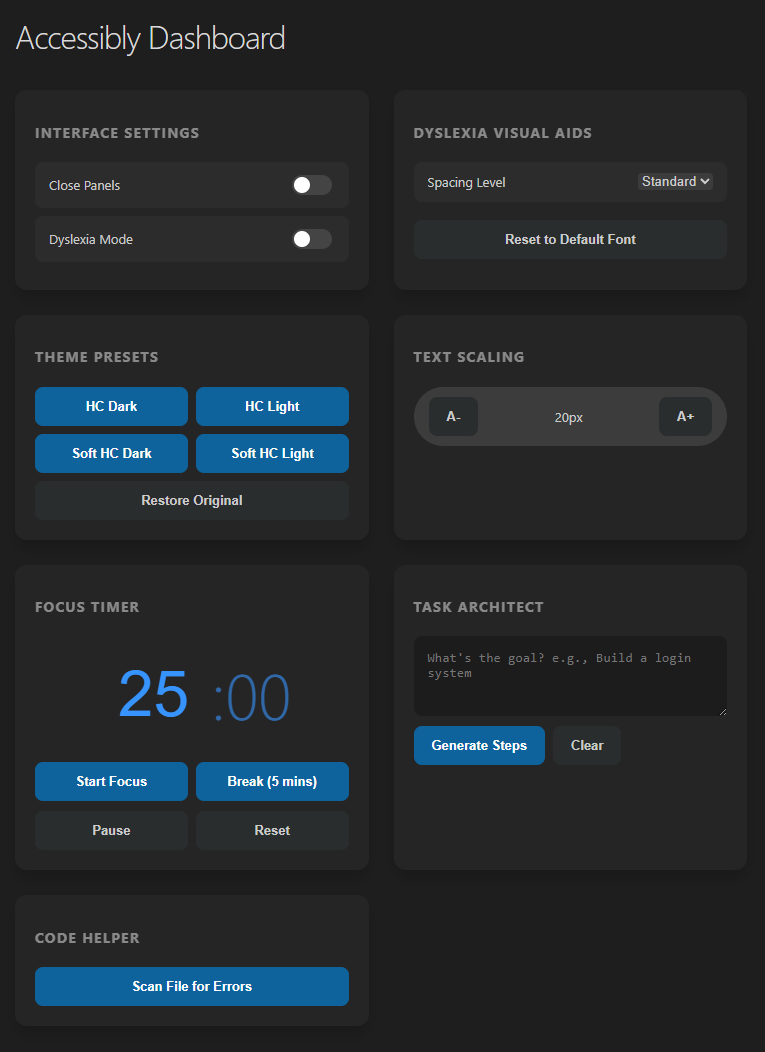
\includegraphics[width=1\linewidth, alt={}] {logos/Final.png}
    \caption{Final UI design.}\label{fig:finalui}
\end{figure}

\subsection{Evaluation and Methodology}

\subsubsection{Ethical Considerations}
Since this project involves human participants and also targets a vulnerable population, ethical considerations are 
paramount. The study will adhere to the following ethical guidelines:
\begin{itemize}
    \item \textbf{Informed Consent:} All participants will have the study fully explained to them, including the purpose, procedures. 
    \item \textbf{Confidentiality:} No names or personally identifiable information will be collected. Including information about the participants' neurodivergent status.
    \item \textbf{Voluntary Participation:} Participation in the study will be entirely voluntary, with no penalties for withdrawal at any stage.
\end{itemize}

\subsubsection{Experimental Design}
This study employs a \textit{within-subjects comparative design}, where each participant acts as their own control. This design is particularly effective for \gls{neurodivergent} research as it accounts for the high degree of individual variance in cognitive processing styles \cite{verma2025differences}. Participants will perform two standardised programming tasks: a project-planning phase and a debugging phase.

\begin{enumerate}
    \item \textbf{Control Condition:} Tasks are performed using a standard \gls{IDE} installation.
    \item \textbf{Experimental Condition:} Tasks are performed using the \gls{IDE} equipped with the Accessible Plugin features (Minimalist Toggle, Task Architect, and Visual Styler).
\end{enumerate}

To mitigate the \textit{carry-over effect} (where learning from the first task makes the second easier), the order of conditions will be counterbalanced, and task sets of equivalent \gls{IL} will be used across both conditions.

\subsubsection{Quantitative and Qualitative Frameworks}
To evaluate the efficacy of the plugin in reducing \gls{EL} and supporting \gls{executive_dysfunction}, two validated instruments will be administered.

\textbf{NASA Task Load Index (\gls{NASATLX})}


The \gls{NASATLX} is a multidimensional assessment tool used to quantify perceived workload. It is uniquely suited for this study as it allows for the isolation of specific cognitive pressures. While all six subscales will be measured to ensure a comprehensive view, the analysis will focus specifically on four key dimensions:

\begin{itemize}
    \item \textbf{Mental Demand:} To assess if the Task Architect successfully reduces the executive function tax required for project initiation.
    \item \textbf{Performance:} To measure the user's self-perception of success in the face of syntax errors or logic bugs.
    \item \textbf{Effort:} To quantify the total mental resources required to reach the goal.
    \item \textbf{Frustration:} Critical for \gls{neurodivergent} populations, this measures the emotional cost of switching between tasks and sensory overwhelm.
\end{itemize}

To evaluate the cognitive and physical demands of both interfaces, a NASA Task Load Index (\gls{NASATLX}) was administered to all participants ($N=5$).
I calculated both the Raw TLX ($r$-score) and the Weighted TLX ($w$-score) to account for individual differences in workload perception. 
The weighting factors were determined by the most important criteria, with Mental Demand (5) and Frustration (4) identified as the primary contributors to workload 
 in this task environment. Factors such as Temporal Demand and Physical Demand were weighted lower, reflecting their lesser impact on the overall workload in this context.

\begin{table}[h]
\centering
\caption{\gls{NASATLX} Weighting Factors}
\begin{tabular}{@{}p{1cm}p{1cm}p{1cm}p{1cm}p{1cm}p{1cm}@{}} % Fixed width for even spacing
\toprule
\textbf{MD} & \textbf{PD} & \textbf{TD} & \textbf{PF} & \textbf{EF} & \textbf{FR} \\ \midrule
5           & 1           & 0           & 3           & 2           & 4           \\ \bottomrule
\end{tabular}
\end{table}
\textbf{System Usability Scale (\gls{SUS})}


To assess the reliability and integration of the tool, the \gls{SUS} will be administered following the Experimental Condition. The \gls{SUS} is a 10-item questionnaire using a 5-point Likert scale, providing a global view of system usability. 

In the context of this study, the \gls{SUS} serves two primary purposes:
\begin{enumerate}
    \item \textbf{Integration Assessment:} Identifying if the \textit{Minimalist Toggle} feels like a seamless part of the workflow or an added complexity.
    \item \textbf{Confidence and Learnability:} Measuring the activation energy required to use the \gls{AI} features. For a developer experiencing \gls{task_paralysis}, a tool that is perceived as irritating to use (Item 8) or complex (Item 2) would be counter-productive.
\end{enumerate}

\subsubsection{Data Collection and Analysis}
In addition to the questionnaires, the study will record \textit{Time-on-Task} (to measure efficiency) and use a \textit{Think-Aloud Protocol}. This qualitative approach will capture real-time instances of \glspl{state_recovery_cost} following an interruption, providing insight into how the \gls{AI} \gls{scaffolding} supports the developer in regaining \gls{hyperfocus}.

\newpage